\documentclass[11pt]{article}
\usepackage[latin1]{inputenc}
\usepackage{a4wide}
\usepackage{amsmath}
\usepackage{amsfonts}
\usepackage{amssymb}
\usepackage{graphicx}
\usepackage{enumerate}
\usepackage{epstopdf}
\usepackage{float}
\usepackage{multicol}
\usepackage{hyperref}
\epstopdfsetup{outdir=./images/}

\title{Natural Computing, Assignment 1}
\author{Pauline Lauron - s1016609 \and Dennis Verheijden - s4455770 \and Joost Besseling - s4796799}
\begin{document}
	\maketitle
	
	\section{}
	Due to no eliteness, we can treat the best member as any other member in the pool.
	
	\begin{enumerate}[(a)]
		\item There are 100 individuals, with a mean of 76. That means that the total size of the roulette wheel will be 7600. The current best member has a fitness of 157, so it will occupy $\frac{157}{7600}$th of the roulette wheel. This means that it has roughly a $2\%$ chance of being selected. If we select 100 members, we expect to select the best member $\frac{157}{7600} * 100 \approx 2 $ times.
		
		\item The chance that we don't select the fittest member is $1 - \frac{157}{7600}$. So the chance that we never select it is $\left(1 - \frac{157}{7600}\right)^{100} \approx 0.124$.
	\end{enumerate}

	\section{}
	
	The fitness function is \[ f(x) = x^2. \]
	
	The members of the pool are $x=3, x=5, \text{and} x=7$. So the total fitness is $3^2 + 5^2 + 7^2 = 83$. The chance to select each individual is: 
	\begin{itemize}
		\item[$x=3:$] $9/83 \approx 0.108$,
		
		\item[$x=5:$] $25/83 \approx 0.301$,
		
		\item[$x=5:$] $49/83 \approx 0.590$.
		 
	\end{itemize}

	When using the alternative selection function 
	\[
		f_1(x) = x^2 + 8,
	\] 
	
	the total fitness is $83 + 24 = 107$ and
	we obtain the following results: 
	
		\begin{itemize}
		\item[$x=3:$] $17/107 \approx 0.159$,
		
		\item[$x=5:$] $33/107 \approx 0.308$,
		
		\item[$x=5:$] $57/107 \approx 0.533$.
		
	\end{itemize}

We can see that the second function yields a lower selection pressure. This is because the relative boost of 8 is much higher for the less fit individuals. It almost doubles the fitness of the $x=3$ individual, and only amounts to a $0.16$-th increase in fitness of the $x=7$ individual.

\section{}
\begin{enumerate}[(a)]
\item When running the algorithm with $n=100$ for 1500 iterations, we can observe the result found in figure \ref{fig:mc}. We can see that the Monte-Carlo search as specified in the assignment did not find the optimal solution.

\item Running the algorithm ten times, the algorithm finds the optimal solution 0 times.

\end{enumerate}

\begin{figure}[H]
\centering
\includegraphics[width=0.75\textwidth]{images/monte_carlo.eps}
\caption{Monte Carlo Search for the Counting Ones problem, ran 10 times.}
\label{fig:mc}
\end{figure}

\section{}
\begin{enumerate}[(a)]
\item When running the (1+1)-GA algorithm for the Counting Ones problem, we found the results from figure \ref{fig:ga}.
\item As we can observe from our results, the algorithm found the optimum 10 times out of 10 runs.
\item If we compare these results to those of the Monte-Carlo algorithm, we can easily see that the Genetic Algorithm is a significant improvement, as the Monte-Carlo algorithm did not find the optimum once and the GA algorithm every time.
\end{enumerate}

\begin{figure}[H]
\centering
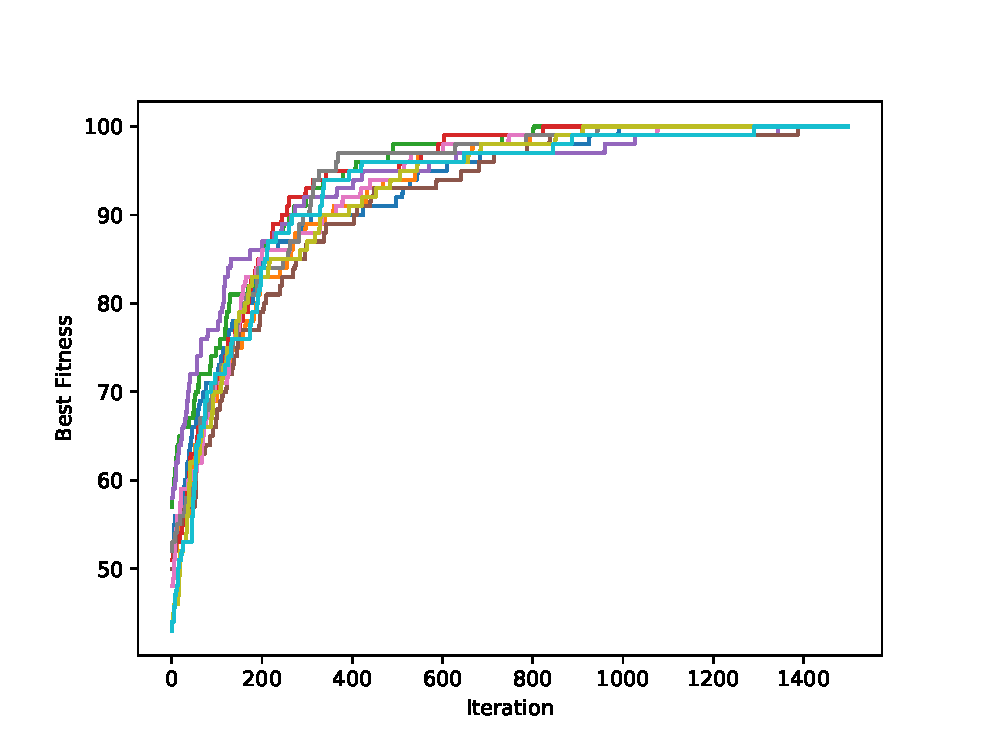
\includegraphics[width=0.75\textwidth]{images/ga.eps}
\caption{(1+1)-GA for the Counting Ones problem, ran 10 times.}
\label{fig:ga}
\end{figure}

\section{}
Suitable function : $F = \{\wedge,\rightarrow, \vee,\leftrightarrow \}$
\newline Terminal set : $T = \{x,y,z,true\}$
\newline S-expression : $ (\rightarrow (\land\ x\ true)(\lor (\lor\ x\ y)(\leftrightarrow z(\land\ x\ y))) $

\section{}
For this exercise, we had to make some changes to the primitive function set. 
First, $\log{0} = -\infty$, we change this such that $\log{0} = 0$. The function \textit{exp} grows exponentially, in order to prevent overflows, we limit it to a maximum value. Finally, we changed \textit{div}, since division by zero is not defined. We changed this by returning 0 if the denominator was zero. These functions are called the protected versions of their primitives.

For the implementation of this assignment we used the python module \texttt{DEAP}. For the tree structure we used a \texttt{genHalfAndHalf} tree, since we think it has more flexibility than using a \textit{grown} or \textit{full} tree. 

In figure \ref{fig:best_fitness}, we see the best of generation fitness per generation. What we can observe from this figure and the output of the algorithm is that the best solution has a \textit{-sum of absolute errors} of $-0.02$, which is pretty good, but not a perfect fit. We hypothesize that a perfect solution is hard to achieve with the current parameters for a number of reasons. 

When looking at the figure, one may note that the algorithm could not find a solution within 50 generations. However, it kept (marginally) improving. So giving it more time could lead to a better solution. Another hypothesis is that the given outputs are not actually generated by a function that can be constructed using our primitive set, so we are instead approximating the best approximation. A solution to speed up the search may be to allow mutations, in that way we search a bigger space. We did a preliminary test, which converged on an error of $-0.0008$ after 100 generations, so we can see that this speeds up the search.

In figure \ref{fig:best_size}, we see the best of generation size per generation. The size is defined by the number of elements in the expression tree. From this figure, we may observe that the best solution of the algorithm does not necessarily have to grow in size to improve. Although we can see a tendency to grow. This might be caused by the fact that a more complex solution leads to a better approximate fit.

After repeating this experiment a 100 times (figure \ref{fig:best_fitness2}-\ref{fig:best_size2}), we believe to have found a possible solution. The algorithm managed to find an individual whose error was $-8.68353e-16$, which is near $0$. This leads us to the belief that random restarts are somewhat the key to the solution (in this case). We believe that this solution may eventually be found by any run given enough time and such that mutations are allowed.

The function that achieved this error is the following:

\begin{verbatim}
add(mul(add(x, mul(add(mul(x, x), x), x)), x), x)
\end{verbatim}

Interestingly, after this solution was found, equivalent but longer solutions are also found. They are then added since there is no penalty for size, and the Hall of Fame adds equally fit individuals as well. 

One such function is the following:

\begin{verbatim}
mul(add(add(x, mul(x, x)), protected_div(sub(x, x), mul(x, mul(x, x)))), add(mul(x, x),
cos(protected_log(protected_div(mul(protected_exp(sub(add(x, mul(x, x)), sin(mul(add(x, 
mul(x, x)), sin(sin(sub(x, x))))))), sin(sin(protected_log(protected_div(mul(x, x), 
sub(mul(x, x), x)))))), sub(sub(x, x), x))))))
\end{verbatim}





\begin{multicols}{2}
\centering
\begin{figure}[H]
\includegraphics[width=0.45\textwidth]{images/genetic_best_fitness.eps}
\caption{Best of generation fitness per generation.}
\label{fig:best_fitness}
\end{figure}
\begin{figure}[H]
\includegraphics[width=0.45\textwidth]{images/genetic_best_size.eps}
\caption{Best of generation size per generation.}
\label{fig:best_size}
\end{figure}
\end{multicols}
\pagebreak

\begin{multicols}{2}
\centering
\begin{figure}[H]
\includegraphics[width=0.45\textwidth]{images/genetic_best_fitness2.eps}
\caption{Best of generation fitness per generation.}
\label{fig:best_fitness2}
\end{figure}
\begin{figure}[H]
\includegraphics[width=0.45\textwidth]{images/genetic_best_size2.eps}
\caption{Best of generation size per generation.}
\label{fig:best_size2}
\end{figure}
\end{multicols}


\end{document}